\section{Experimental analysis}
\raziel{Experimental analysis: proposed outline.}

\begin{figure}[th]
	\begin{center}
		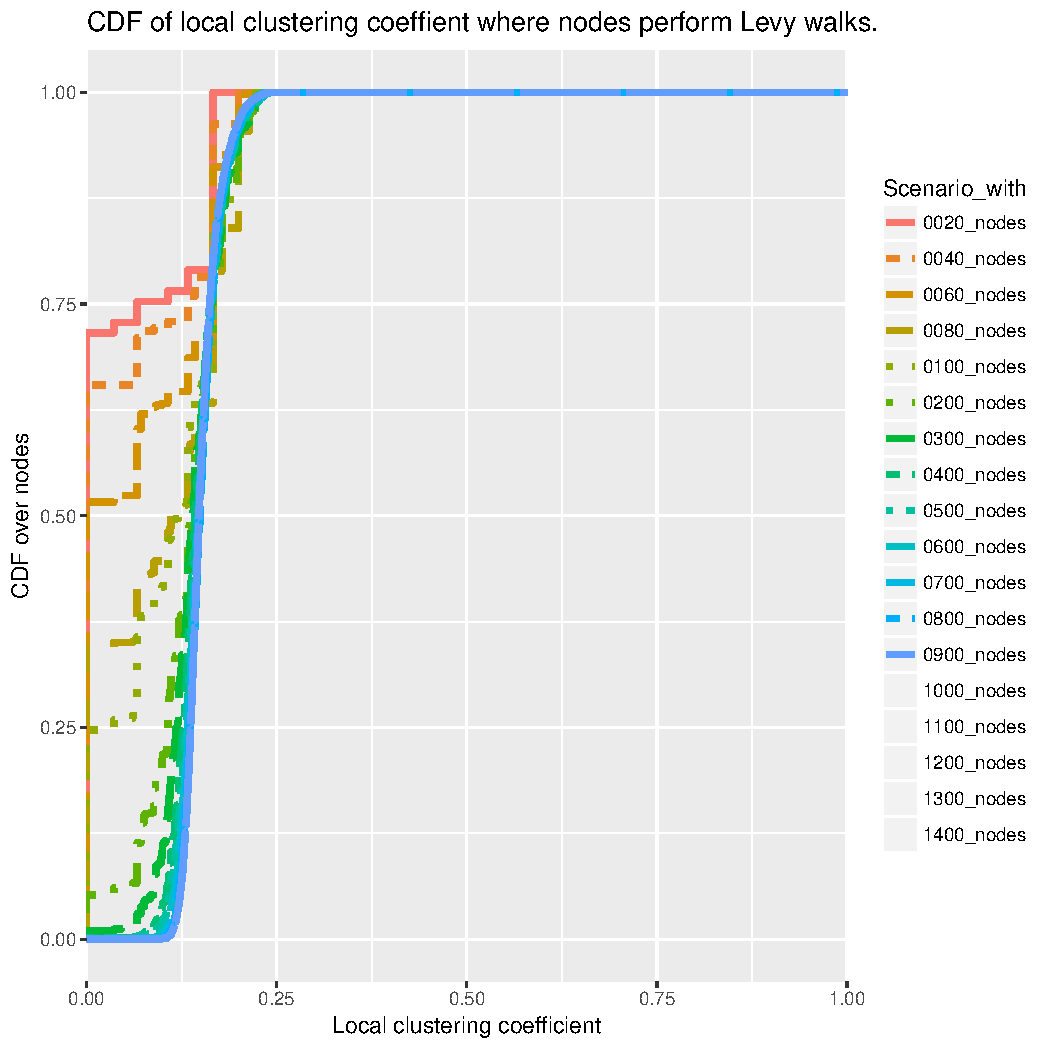
\includegraphics[page=1, scale=0.45, trim = 20mm 0mm 0 0]{figures/preliminary_results/cc.pdf}
		\caption{ \labfigure{lcc}}
	\end{center}
\end{figure}

\begin{figure}[th]
	\begin{center}
		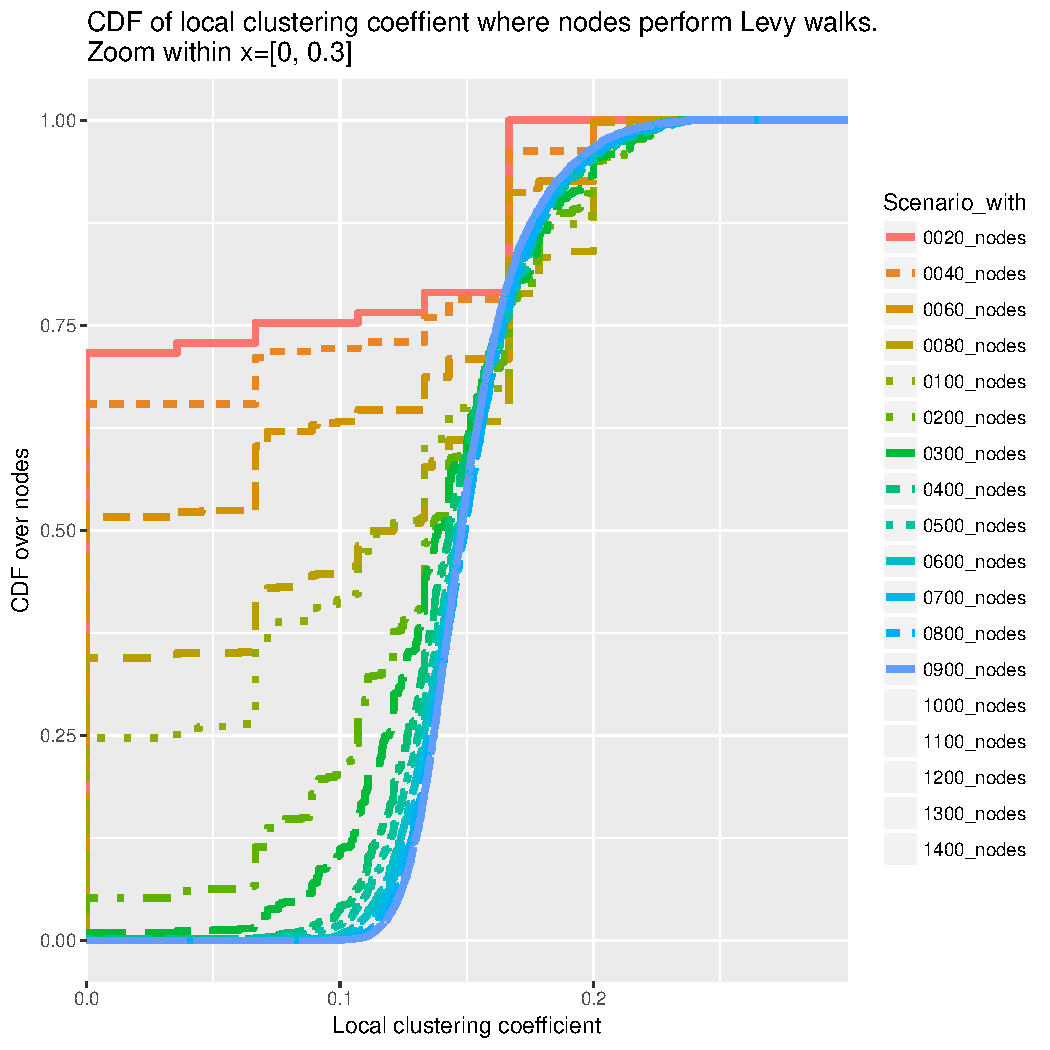
\includegraphics[page=1, scale=0.45, trim = 20mm 0mm 0 0]{figures/preliminary_results/cc_zoom.pdf}
		\caption{ \labfigure{lcc-zoom}}
	\end{center}
\end{figure}

\begin{figure}[th]
	\begin{center}
		
\includegraphics[page=1, scale=0.45, trim = 20mm 0mm 0 0]{figures/preliminary_results/density.pdf}
		\caption{ \labfigure{density}}
	\end{center}
\end{figure}

\begin{itemize}
\item Justification: MANETs fit well in such realistic scenarios where potentially there is no infrastructure.
\item \textit{TODO: Find a wireless topology (from realistic trace, protest or concert?) to emphasize the characterization of PoI}
\item we characterize a PoI in zones according to the acceleration of nodes

\begin{itemize}
	\item zone $Z_{sparse}$ with low density of nodes and high acceleration: where the Local Clustering Coefficient (LCC) of nodes is closer to 0
	\item zone $Z_{dense}$ with high density of nodes and low acceleration: with LCC of nodes closer to 1
\end{itemize}

\item Broadcast protocols in MANETs rely on the information available on each node to perform forwarding decisions (GPS coordinates, collisions in MAC, etc.)
\item We use the acceleration of nodes as well as LCC (both local information) in broadcast algorithms for MANETs where nodes perform (truncated) Levy walks
	\begin{itemize}
		\item let $z(l,a)=c(l)-n(a)$ be a function to decide if a node belongs to $Z_{dense}$ or $Z_{sparse}$
		\item $c(l) \exists [0,1]$ is the LCC
		\item $n(a) \exists [0,1]$ is a normalization of the node acceleration. \textit{TODO: find out trigonometric identity to map nodes acceleration within $[0,1]$}
		\item function $z \exists [-1, 1]$
		\begin{itemize}
		\item the more positive $f$ the higher the probability that a node is at $Z_{dense}$
		\item the more negative $f$, the higher the probability that a node is at $Z_{sparse}$
		\item $l$ is the list of two-hop neighbors; result of exchange of control messages
		\end{itemize}
	\end{itemize}

\item Our policy of adaptation as well as the interoperability mechanism (between broadcast algorithms) relay on 2 factors: LCC and nodes acceleration. \textit{TODO: highlight that no external entity is needed}. \textbf{Why LCC and acceleration.} both factors adapt themselves as needed. Here, getting LLC requires a periodic exchange of control messages; price to pay even in broadcast algorithms that do not rely in overlays. On the other hand, such exchange of beacons take place when a source node decides to disseminate a will of change (look at the algorithm of our basic policy of adaptation).

\end{itemize}

\raziel{Take into account the acceleration of nodes seems a natural choice to determine the zone where nodes move. On the other hand, for the local clustering coefficient we do require to analyze how this factor behaves in a wireless topology where nodes perform Levy walks.}

\begin{itemize}
	\item Ideally we should use real traces to study the LCC. \textbf{TODO: look for such traces}
	\item We do count with preliminary results to observe how LCC evolves in dynamic scenarios, this is shown in~\reffigure{lcc}, ~\reffigure{lcc-zoom}, ~\reffigure{density}; here there is a description of such experiments:
	\begin{itemize}
		\item on each experiment there is a fixed number of nodes; such number varies from 20 to 1400
		\item communication area of $100m^{2}$ remains the same in all experiments
		\item for an experiment $E_{i}$ a mobility trace $T_{i}$ was created where every node performs Levy walks every second with a random velocity between 0m/s to 1m/s; total time on each trace is 30s
		\item transmission range of nodes remains the same for all experiments
	\end{itemize}

\end{itemize}

\raziel{
Takes away at the end of this section:
\begin{itemize}
	\item nodes acceleration and LCC are factors that make sense to determine whether or not nodes are at PoI
	\item assure that LCC is a metric that haven't been explored (at least not explicitly) before to find out opportunities to broadcast in MANETs
	\item we differ from other works that make use of explicit use of thresholds of density
\end{itemize}
}

\raziel{
Other ideas/questions to explore:
\begin{itemize}
	\item is there any other metric in graph theory that nodes can compute in a decentralized manner to improve network performance? or probably propose another policy of adaptation ?
\end{itemize}
}